\documentclass[aspectratio=169]{beamer}
\usetheme[progressbar=frametitle]{metropolis}           % Use metropolis theme
\setbeamertemplate{frame numbering}[fraction]
\metroset{background=dark} % change background theme according to manual

\usepackage{hyperref}
\usepackage{graphicx} % package to use links
\usepackage{xcolor}
\definecolor{aqua}{RGB}{41, 170, 225}

\setbeamercolor{palette primary}{bg=white,fg=black}
\setbeamercolor{background canvas}{parent=palette primary}
\setbeamercolor{normal text}{fg=black}
\setbeamercolor{progress bar}{use=palette primary,fg=aqua}

\setbeamersize{text margin left=1em,text margin right=1em}

%\usecolortheme{crane}

\setbeamersize{text margin left=1em,text margin right=1em}

\newcommand{\SubItem}[1]{
        {\setlength\itemindent{15pt} \item[-] #1}
}

% footnote without number
\newcommand\blfootnote[1]{
    \begingroup
    \renewcommand\thefootnote{}\footnote{#1}
    \addtocounter{footnote}{-1}
    \endgroup
}

% footnote and page number on same line
\setbeamertemplate{footline}{}

\setbeamertemplate{logo}{
    \usebeamercolor[fg]{footline}
    \usebeamerfont{page number in head/foot}
    \usebeamertemplate*{frame numbering}
}

\usepackage[nolist]{acronym}

\usepackage[backend=biber, style=authoryear]{biblatex}
%\usepackage[style=authortitle,backend=biber]{biblatex}
% alternatively you can add the citaion into the footer with \footcite{AuthorKey}
\addbibresource{mybibfile.bib}
\AtBeginBibliography{\small}

%\usecolortheme{crane}

\title{Human energy balance model to determine upper limit temperature and humidity conditions for the use of electric fans}
\subtitle{When electric fans can be used during heatwaves?}
\date{\today}
\author[Tartarini, Schiavon, Arens, Huizenga] % (optional, for multiple authors)
{Federico~Tartarini\inst{1}, Stefano~Schiavon\inst{2}, Edward~Arens\inst{2}, Charlie~Huizenga\inst{2} \\[2ex] 
\includegraphics[width=4cm]{figures/sinberbest.png}}
\institute{
    \inst{1}%
    SinBerBEST, Berkeley Education Alliance for Research in Singapore, SG
    \and
    \inst{2}%
    Center for the Built Environment, University of California Berkeley, USA
}

\begin{document}
    \maketitle

    %! Author = sbbfti
%! Date = 10/06/2020

\section*{Nomenclature}
\renewcommand{\baselinestretch}{0.75}\normalsize
\begin{acronym}[longest]

    \acro{t-db}[$t_{db}$]{dry-bulb air temperature\acroextra{, $^{\circ}$C}}
    \acro{ti}[$t_{i}$]{indoor air temperature\acroextra{, $^{\circ}$C}}
    \acro{tout}[$t_{out}$]{outdoor air temperature\acroextra{, $^{\circ}$C}}
    \acro{t-op}[$t_{o}$]{operative air temperature\acroextra{, $^{\circ}$C}}
    \acro{t-cl}[$t_{cl}$]{clothing temperature\acroextra{, $^{\circ}$C}}
    \acro{tg}[$t_{g}$]{globe temperature\acroextra{, $^{\circ}$C}}
    \acro{rh}[$RH$]{relative humidity\acroextra{, \%}}
    \acro{v}[$V$]{average air speed\acroextra{, m/s}}
    \acro{t-r}[$\overline{t_{r}}$]{mean radiant temperature\acroextra{, $^{\circ}$C}}
    \acro{clo}[$I_{cl}$]{total clothing insulation\acroextra{, clo}}
    \acro{i-cl}[$i_{cl}$]{permeation efficiency of water vapor through the clotying layer}
    \acro{met}[$M$]{rate of metabolic heat production\acroextra{, W/m\textsuperscript{2}}}
    \acro{work}[$W$]{rate of mechanical work accomplished\acroextra{, W/m\textsuperscript{2}}}
    \acro{t-sk}[$t_{sk}$]{skin mean temperature\acroextra{, $^{\circ}$C}}
    \acro{t-cr}[$t_{cr}$]{core mean temperature\acroextra{, $^{\circ}$C}}
    \acro{r-cl}[$R_{cl}$]{thermal resistance of clothing\acroextra{, m\textsuperscript{2}K/W}}
    \acro{r-e-cl}[$R_{cl}$]{evaporative heat transfer resistance of clothing layer\acroextra{, m\textsuperscript{2}kPa/W}}
    \acro{f-cl}[$f_{cl}$]{clothing area factor $A_{cl}/A_{body}$\acroextra{, m\textsuperscript{2}K/W}}
    \acro{h}[$h$]{sum of convective $h_{c}$ and radiative $h_{r}$ heat transfer coefficients\acroextra{, W/(m\textsuperscript{2}K)}}
    \acro{h-r}[$h_{r}$]{linear radiative heat transfer coefficient\acroextra{, W/(m\textsuperscript{2}K)}}
    \acro{h-c}[$h_{c}$]{convective heat transfer coefficient\acroextra{, W/(m\textsuperscript{2}K)}}
    \acro{h-e}[$h_{e}$]{evaporative heat transfer coefficient\acroextra{, W/(m\textsuperscript{2}kPa)}}

    \acro{cl-a}[$A_{cl}$]{clothing surface area\acroextra{, m\textsuperscript{2}}}
    
    \acro{e}[$\varepsilon$]{average emissivity of clothing or body surface}
    \acro{sigma}[$\sigma$]{Stefan-Boltzmann constant\acroextra{, 5.67 x 10\textsuperscript{-8} W/(m\textsuperscript{2}K\textsuperscript{2})}}

    \acro{a-r}[$A_{r}$]{effective  radiation  area  of  the  body\acroextra{, m\textsuperscript{2}}}
    \acro{body-a}[$A_{body}$]{body surface area\acroextra{, m\textsuperscript{2}}}
    \acro{body-w}[$mass$]{body mass\acroextra{, kg}}
    \acro{body-h}[$height$]{body height\acroextra{, m}}

    \acro{pmv}[PMV]{Predicted Mean Vote}
    \acro{ppd}[PPD]{Predicted Percentage of Dissatisfied\acroextra{, \%}}
    \acro{set}[SET]{Standard Effective Temperature\acroextra{, $^{\circ}$C}}
    \acro{ce}[CE]{Cooling Effect\acroextra{, $^{\circ}$C}}

    \acro{BMS}[BMS]{Building Management System}
    \acro{HVAC}[HVAC]{Heating, Ventilation, and Air Conditioning}
    \acro{VAV}[VAV]{Variable Air Volume}
    \acro{AHU}[AHU]{Air Handling Unit}

    \acro{ema}[EMA]{Ecological Momentary Assessment}
    \acro{sdk}[SDK]{Software Development Kit}
    \acro{api}[API]{Application Programming Interface}

    \acro{s-cr}[$S_{cr}$]{rate of heat storage in the core compartment\acroextra{, W/m\textsuperscript{2}}}
    \acro{s-sk}[$S_{sk}$]{rate of heat storage in the skin compartment\acroextra{, W/m\textsuperscript{2}}}
    \acro{s}[$S$]{rate of heat storage in the human body\acroextra{, W/m\textsuperscript{2}}}
    \acro{e-res}[$E_{res}$]{rate of evaporative heat loss from respiration\acroextra{, W/m\textsuperscript{2}}}
    \acro{e-dif}[$E_{dif}$]{rate of evaporative heat loss from moisture diffused through the skin\acroextra{, W/m\textsuperscript{2}}}
    \acro{e-rsw}[$E_{rsw}$]{rate of evaporative heat loss from sweat evaporation\acroextra{, W/m\textsuperscript{2}}}
    \acro{e-sk}[$E_{sk}$]{total rate of evaporative heat loss from skin\acroextra{, W/m\textsuperscript{2}}}
    \acro{e-max}[$E_{max}$]{maximum rate of evaporative heat loss from skin\acroextra{, W/m\textsuperscript{2}}}
    \acro{c-res}[$C_{res}$]{rate of convective heat loss from respiration\acroextra{, W/m\textsuperscript{2}}}
    \acro{c-r}[$C + R$]{sensible heat loss from skin\acroextra{, W/m\textsuperscript{2}}}
    \acro{q-res}[$q_{res}$]{total rate of heat loss through respiration\acroextra{, W/m\textsuperscript{2}}}
    \acro{q-sk}[$q_{sk}$]{total rate of heat loss from skin\acroextra{, W/m\textsuperscript{2}}}
    \acro{w}[$w$]{skin wettedness}
    \acro{w-max}[$w_{max}$]{skin wettedness practical upper limit}
    \acro{m-sweat}[$m_{rsw}$]{rate at which regulatory sweat is generated\acroextra{, mL/h\textsuperscript{2}}}

    \acro{p-sk}[$p_{sk,s}$]{water vapor pressure at skin\acroextra{, kPa}}
    \acro{p-a}[$p_{a}$]{water vapor pressure in ambient air\acroextra{, kPa}}

    \acro{wmo}[WMO]{World Meteorological Organization}
    \acro{who}[WHO]{World Health Organization}
    \acro{cdc}[CDC]{Centers for Disease Control and Prevention}
    \acro{noaa}[NOAA]{National Oceanic and Atmospheric Administration}
    \acro{epa}[EPA]{United States Environmental Protection Agency}
    \acro{iea}[IEA]{International Energy Agency}
    \acro{un}[UN]{United Nations}

\end{acronym}
\renewcommand{\baselinestretch}{1}\normalsize


    \begin{frame}{Aim}
        To determine under which environmental (i.e., \ac{t-db}, \ac{t-r}, \ac{v}, \ac{rh}) and personal factors (i.e., \ac{clo}, \ac{met}) the use of electric fans is beneficial to cool the human body.
    \end{frame}

    \begin{frame}{Background}
        Heatwaves caused more than 166'000 deaths from 1998--2017.

        Thermoregulatory factors, demographics and socioeconomic characteristics, such as age (very young and elderly), pre-existing conditions, low income, homeless, prolonged outdoor activities, and social isolation all play a negative role and increase the heat risk during heatwaves~\cite{WMO2015}
    \end{frame}

    \begin{frame}{Background}
        \begin{itemize}
            \item Electric fans are an effective, energy efficient, and low cost solution to cool people.
            \item They can be used either as an alternative cooling technology or in combination with air conditioning~\cite{Jay2019a, Hoyt2015, Schiavon2008}.
            \item Electric fans remain the most common form of cooling in households~\cite{IEA2018}.
        \end{itemize}
    \end{frame}

    \begin{frame}{Use of Fans}
        National and international guidelines discourage people from using them when indoor air temperatures exceed the skin temperature.

        Previous experimental studies have shown that fans:
        \begin{itemize}
            \item Are beneficial, even when \ac{t-db} exceeds \ac{t-sk}.
            \item Air flow increases heat dissipation via the evaporation of sweating~\cite{Jay2015}.
            \item The maximum \ac{t-db} will depend on \ac{rh}.
        \end{itemize}
    \end{frame}

    \begin{frame}{Jay's model}
        Jay's developed a simplified heat balance model.

        Limitations:
        \begin{itemize}
            \item constant \ac{met} or \ac{clo}
            \item constant \ac{t-sk} and \ac{t-cr}
            \item single air speed 4.5~m/s
        \end{itemize}
    \end{frame}

    \begin{frame}{Objectives}
        Use Gagge's model to estimate heat losses and physiological variables as a function of environmental and personal factors~\cite{Gagge1986}.

        Incorporate the model into CBE thermal comfort tool and pythermalcomfort
    \end{frame}

    \begin{frame}{Methodology - Heat Balance Equation}
        The human body exchanges both sensible and latent heat with its surrounding environment.
        Sensible heat is transferred via conduction, convection and radiation (\acs{c-r} + \acs{c-res}).
        While latent heat loss occurs from the evaporation of sweat (\acs{e-rsw}), moisture diffused through the skin  (\acs{e-dif}), and respiration (\acs{e-res})
        The energy balance in the human body is described by:

        \begin{equation}
            M - W = C + R + E_{sk} + C_{res} + E_{res} + S_{sk} + S_{cr}\label{eq:heat-balance}
        \end{equation}

        \begin{equation}
            E_{s k}=E_{rsw}+E_{dif}
        \end{equation}

        If the exogenous and endogenous heat gains cannot be compensated by heat loss, then both the \ac{s-sk}, and the \ac{s-cr} increase.
    \end{frame}

    \begin{frame}{Data Analysis}
        Assumptions:
        \begin{itemize}
            \item `still air' \ac{v}~=~0.2 m/s.
            \item \ac{t-r} to be equal to \ac{t-db}, \ac{clo}~=~0.5~clo, and \ac{met}~=~1.1~met, unless otherwise specified.
            \item Thermal stress when either of the following parameters reach their maximum value: \ac{w}, skin blood flow, or \ac{m-sweat}.
        \end{itemize}
    \end{frame}

    \begin{frame}{Methodology -- Additional Datasets}
        2017 ASHRAE Handbook--Fundamentals -- the maximum extreme \ac{t-db} and \ac{t-wb} recorded across more than 5000 stations worldwide with a 20 year return period.

        City population data 115 most populous cities in the world from \ac{un} statistic division~\cite{UNdatare88:online}
    \end{frame}

    \begin{frame}{Results}
        \begin{figure}[thb!]
            \centering
            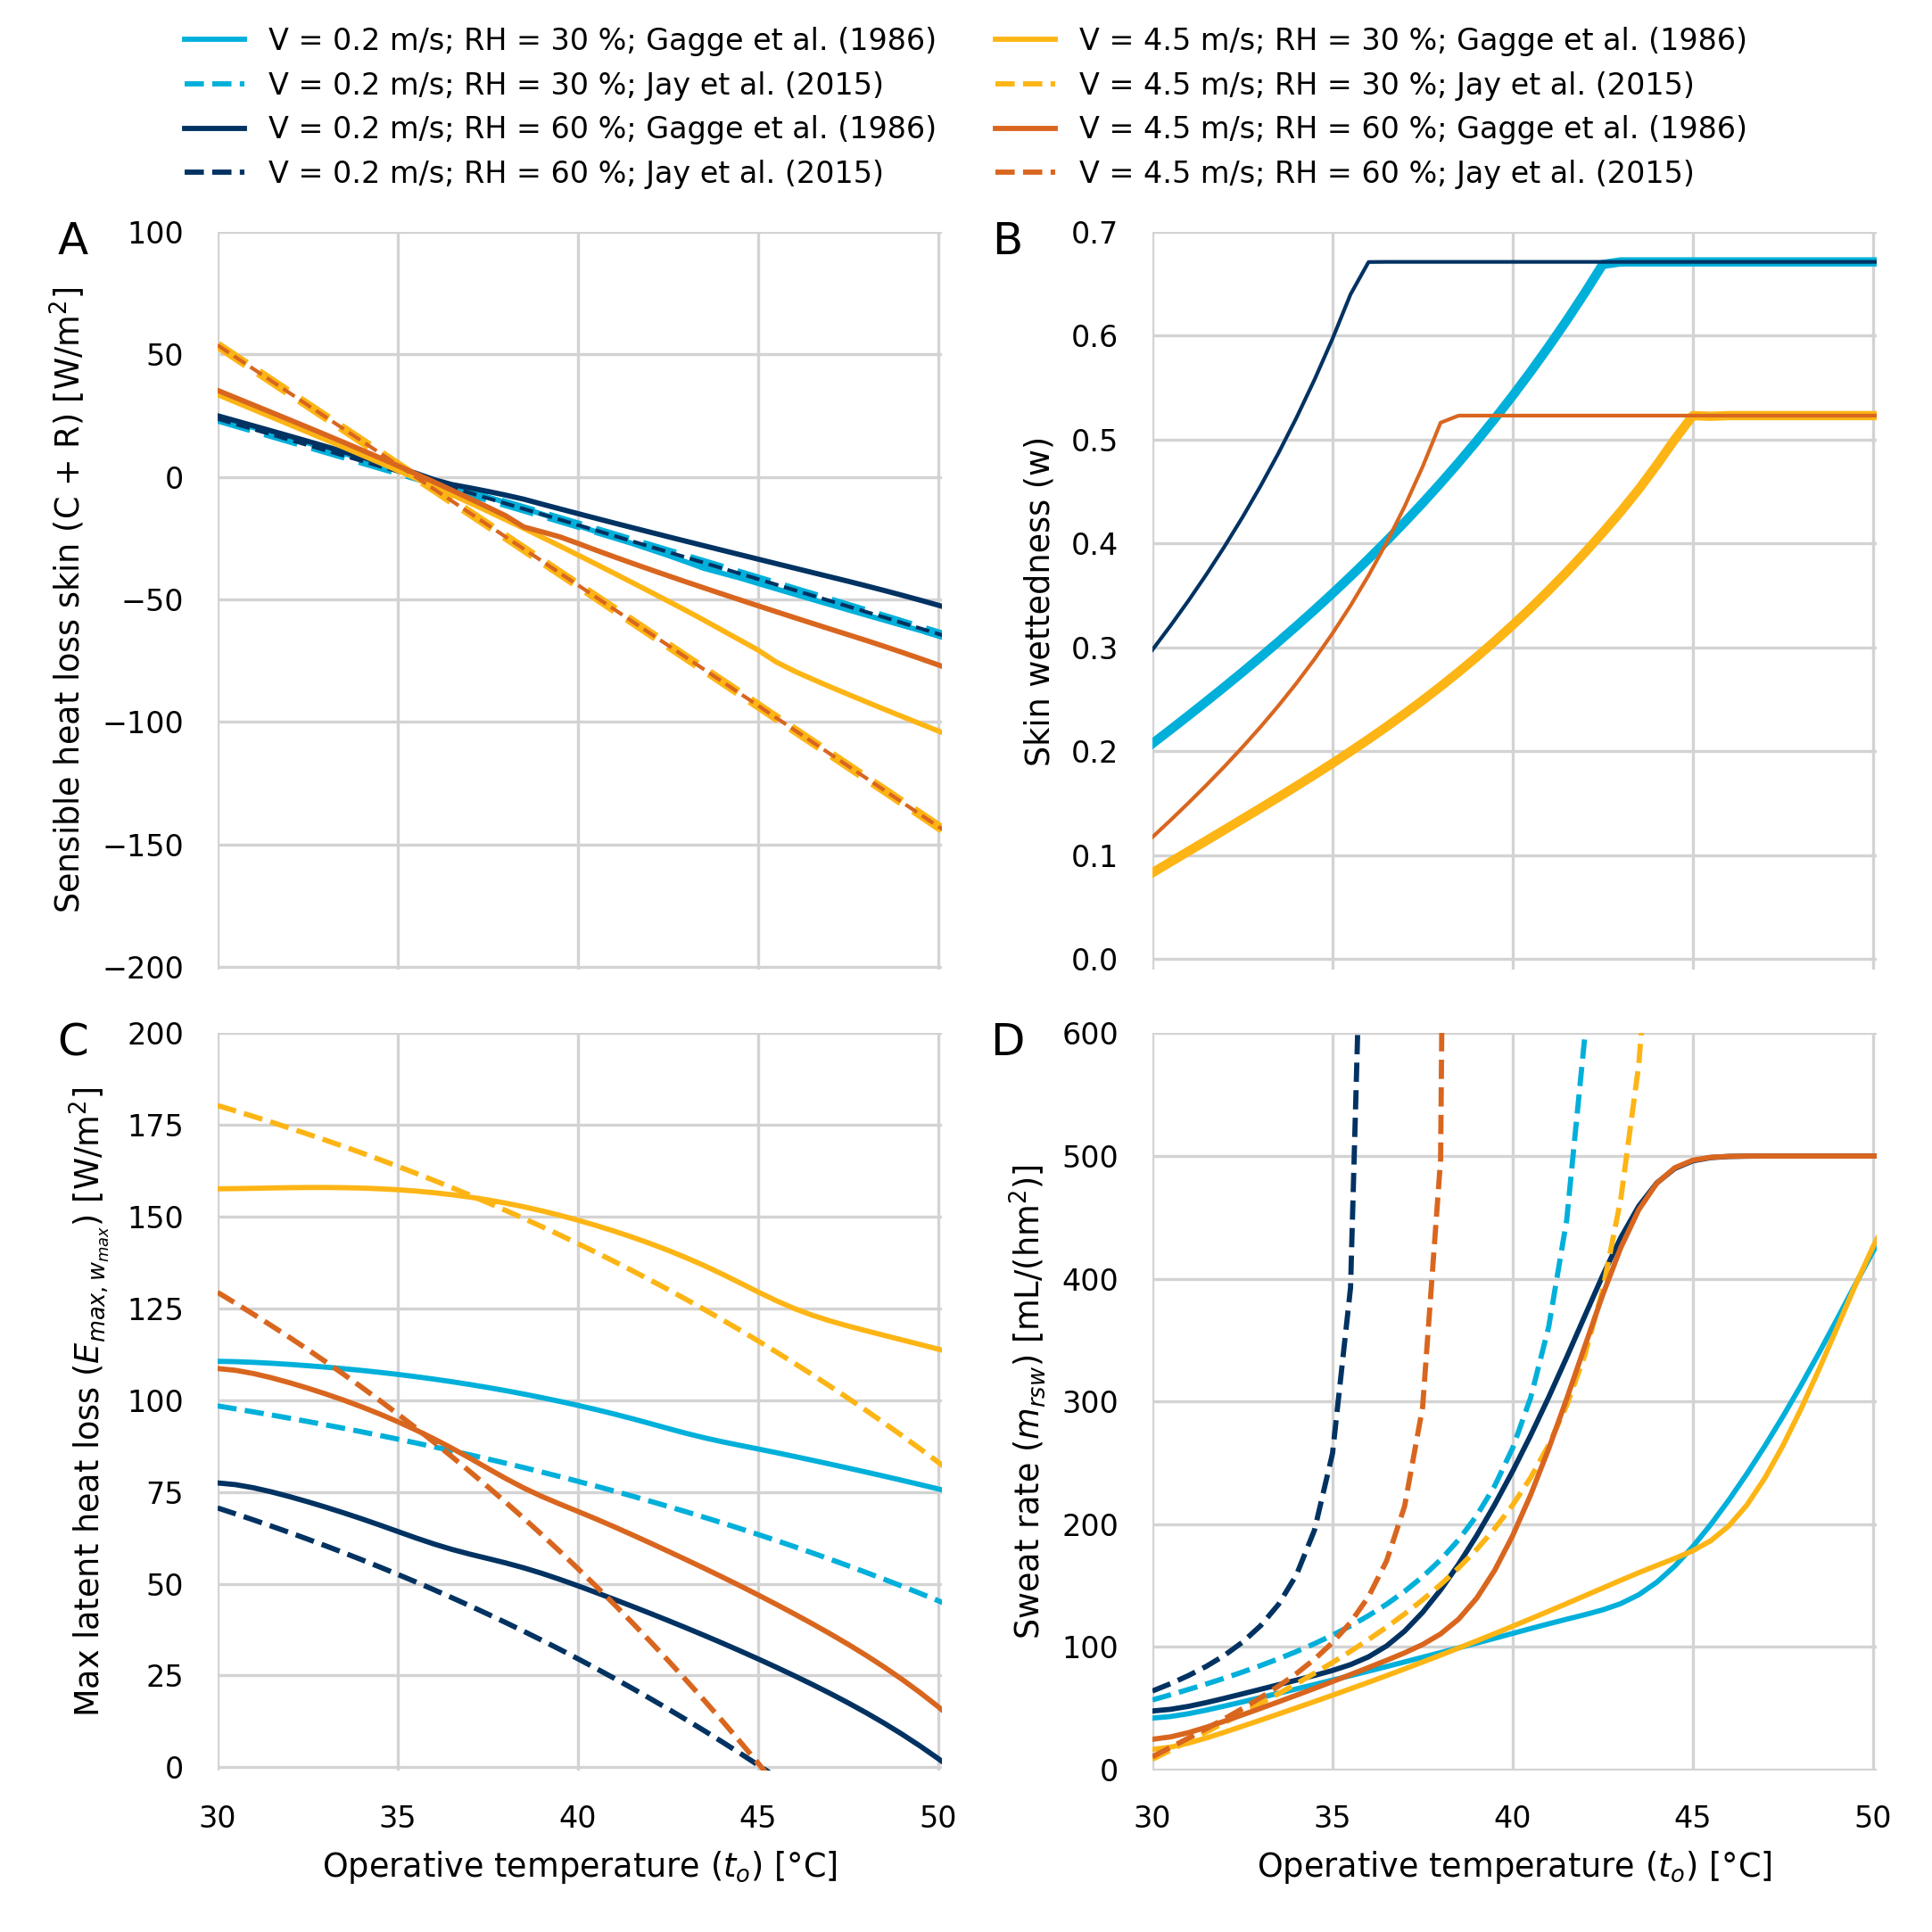
\includegraphics[width=0.5\textwidth]{figures/comparison_models_v2}
            \caption{Results obtained with the energy models proposed by Jay and Gagge.
            Each Figure shows how a variable changes as a function of \ac{t-op} for a set combination of \ac{rh} and \ac{v}.
            Figure: A) \Acf{c-r}.
            B) \Acf{w}.
            C) \Acf{e-max} estimated using \ac{w} = \ac{w-max}.
            D) \Acf{m-sweat}.}
            \label{fig:comparison_models}
        \end{figure}
    \end{frame}

    \begin{frame}{Results}
        \begin{figure}[thb!]
            \centering
            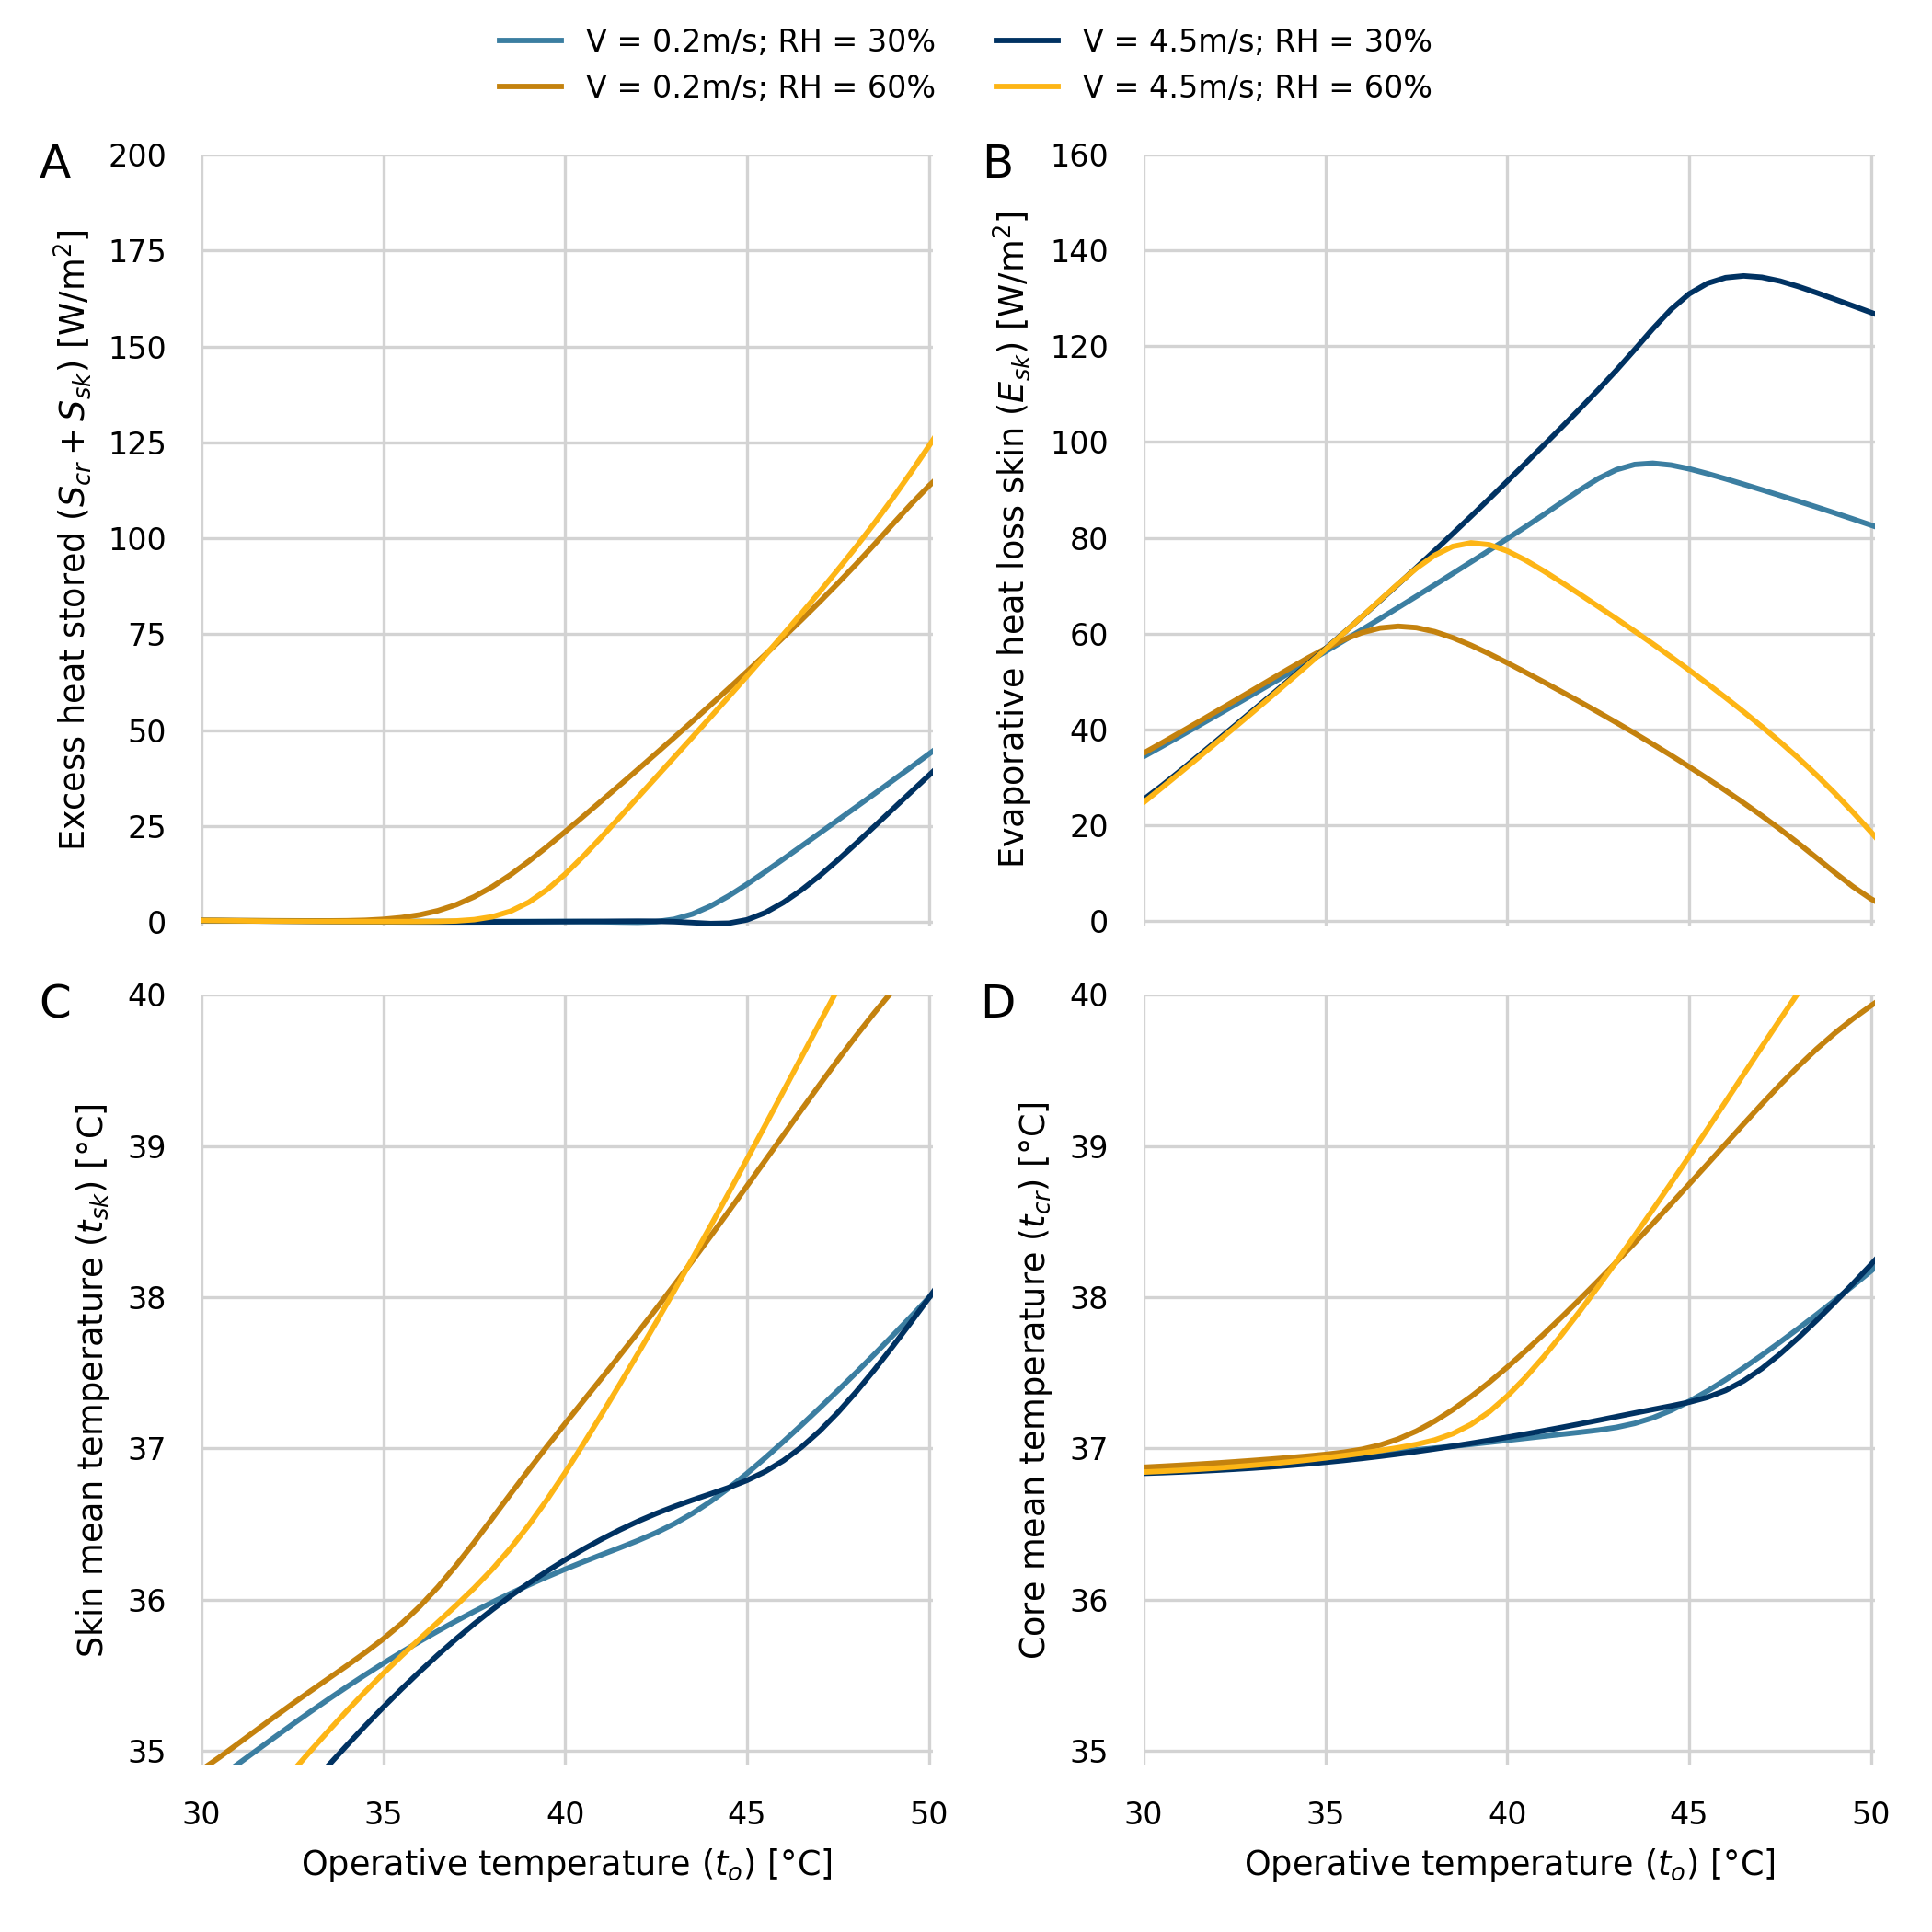
\includegraphics[width=0.5\textwidth]{figures/results_model_2}
            \caption{Results obtained with Gagge energy model.
            Each Figure shows how a variable changes as a function of \ac{t-op} for a set combination of \ac{rh} and \ac{v}.
            Figure: A)  Excess heat stored in the human body, skin and core compartments (\ac{s-sk} + \ac{s-cr}).
            B) \Acf{e-sk}.
            C) \Acf{t-sk}.
            D) \Acf{t-cr}.}
            \label{fig:results_model_2}
        \end{figure}
    \end{frame}

    \begin{frame}{Results}
        \begin{figure}[thb!]
            \centering
            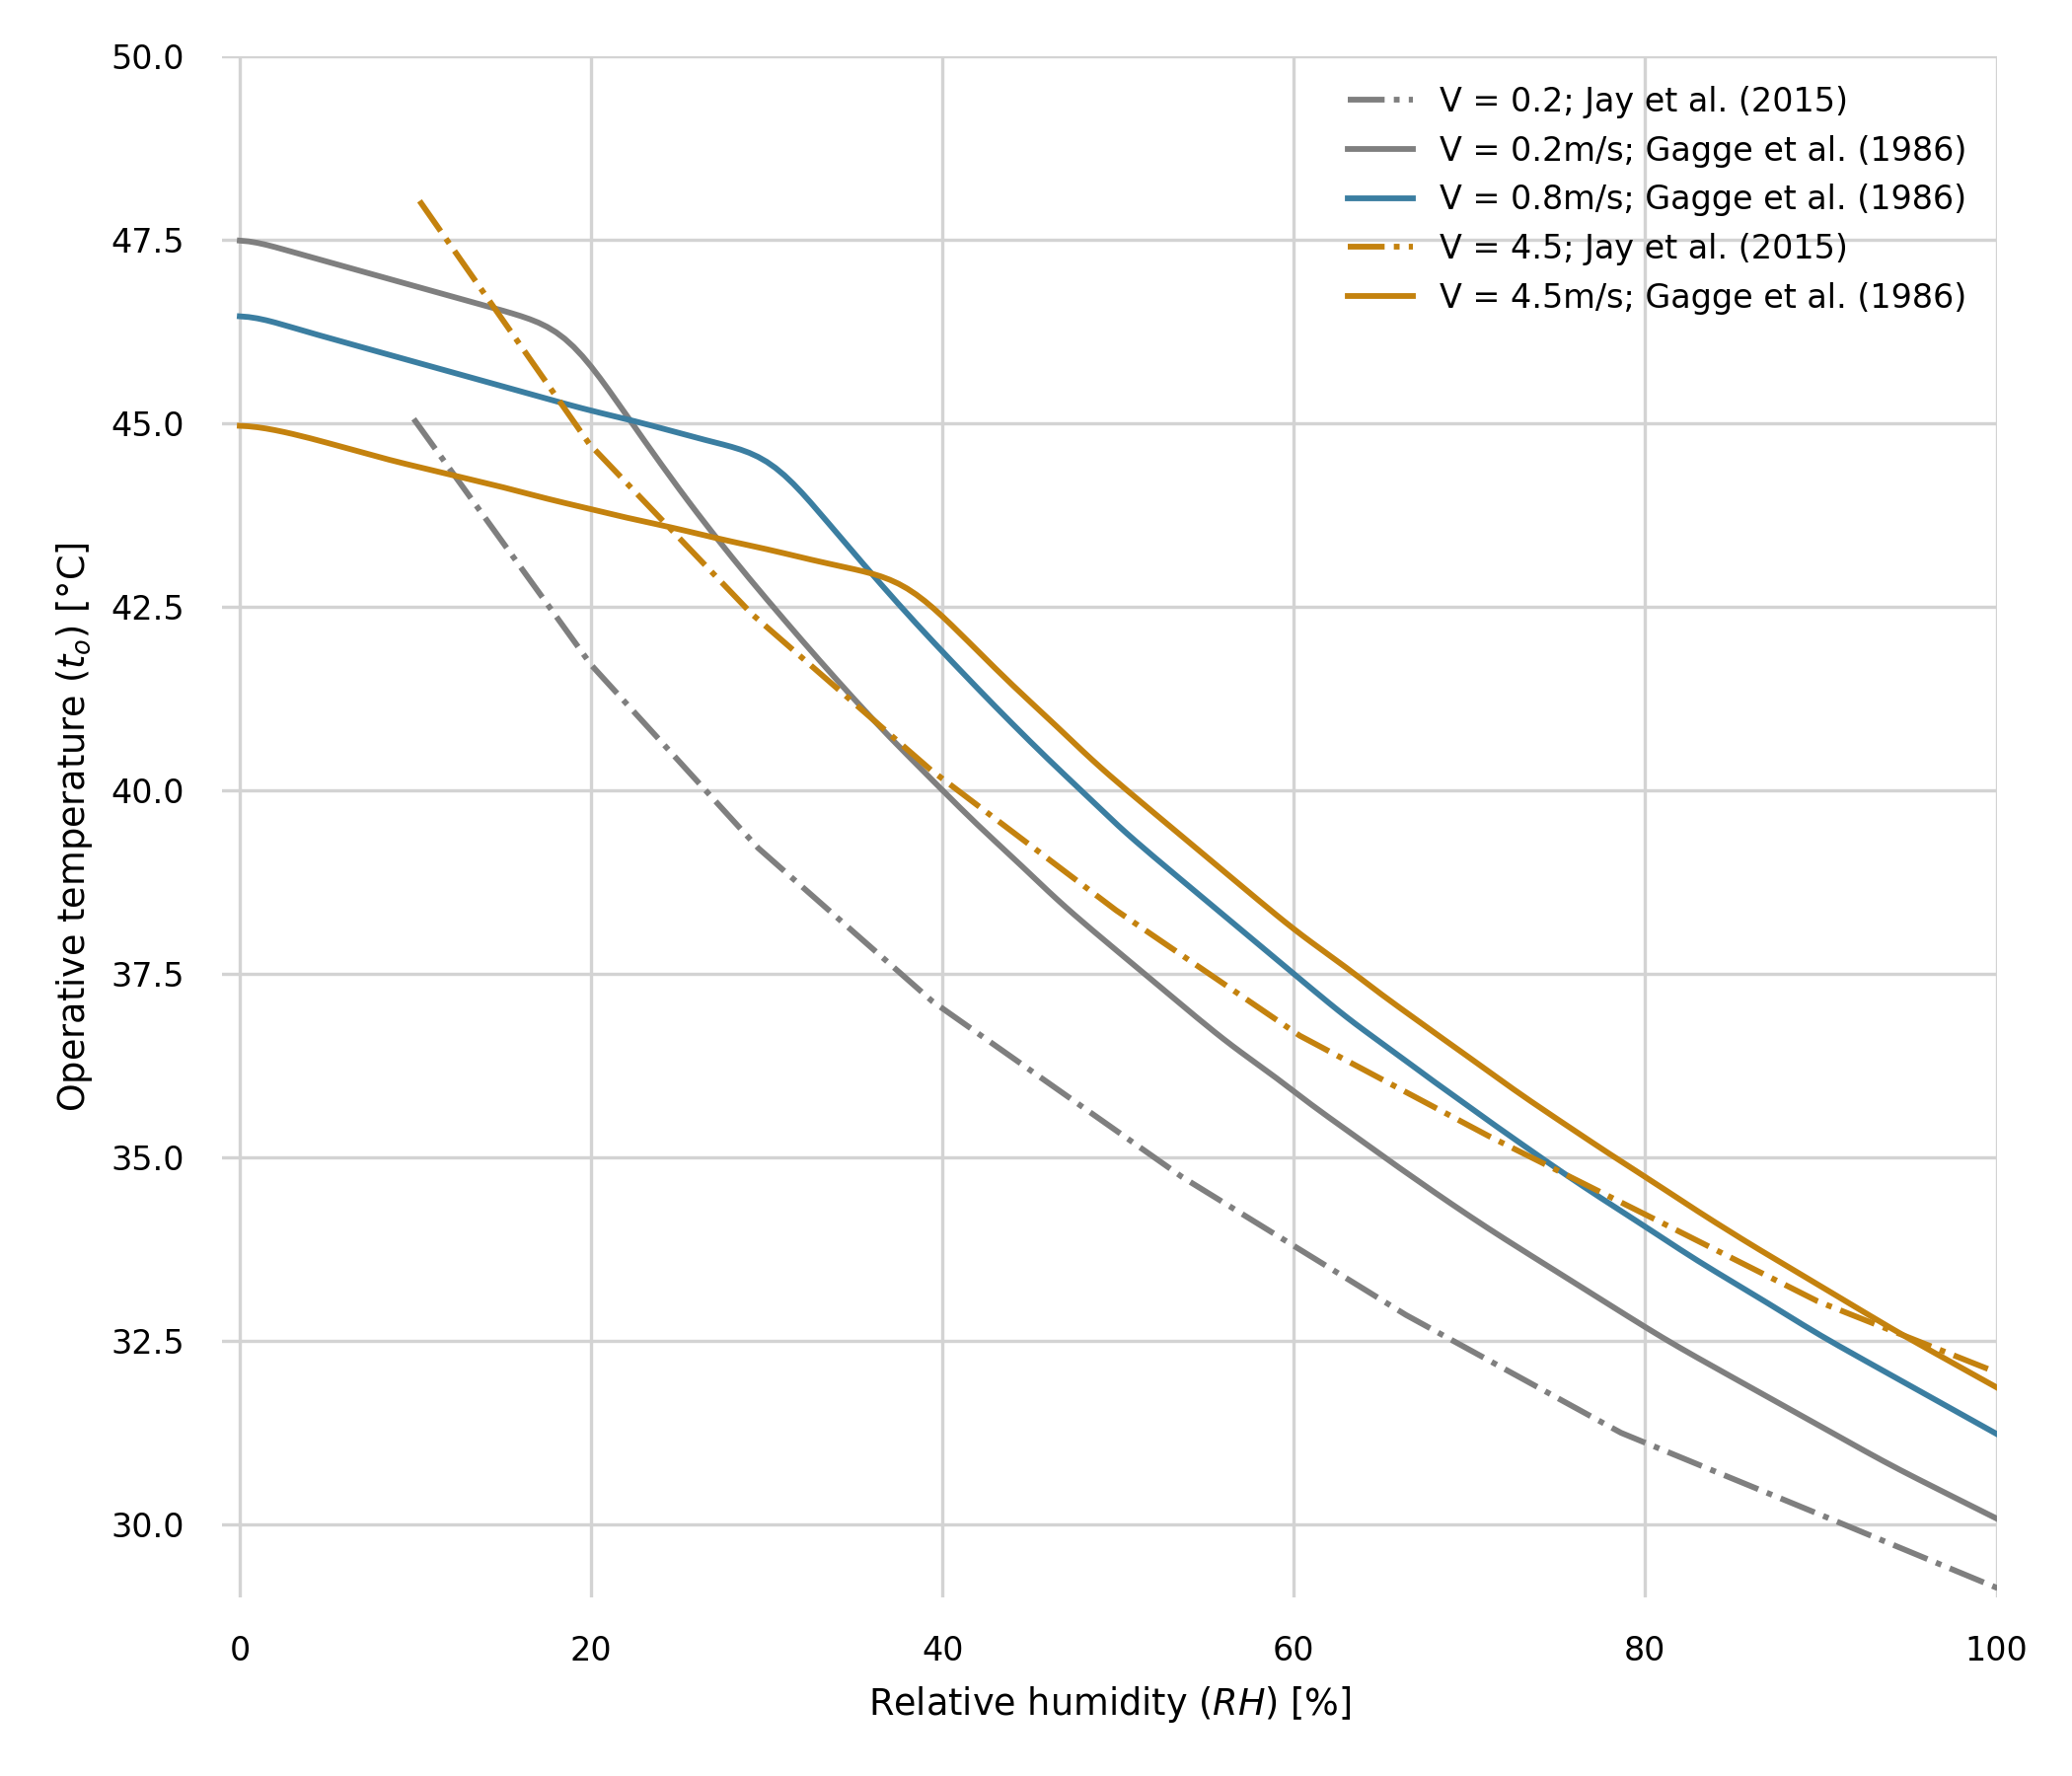
\includegraphics[width=0.6\textwidth]{figures/comparison_air_speed}
            \caption{Predicted limits above which thermal strain is estimated to occur.
            The figure shows the results calculated using the Gagge model and the Jay models.
            Each line demarcates the point above which heat strain is expected to occur.}
            \label{fig:comparison_air_speed}
        \end{figure}
    \end{frame}

    \begin{frame}{Results}
        \begin{figure}[thb!]
            \centering
            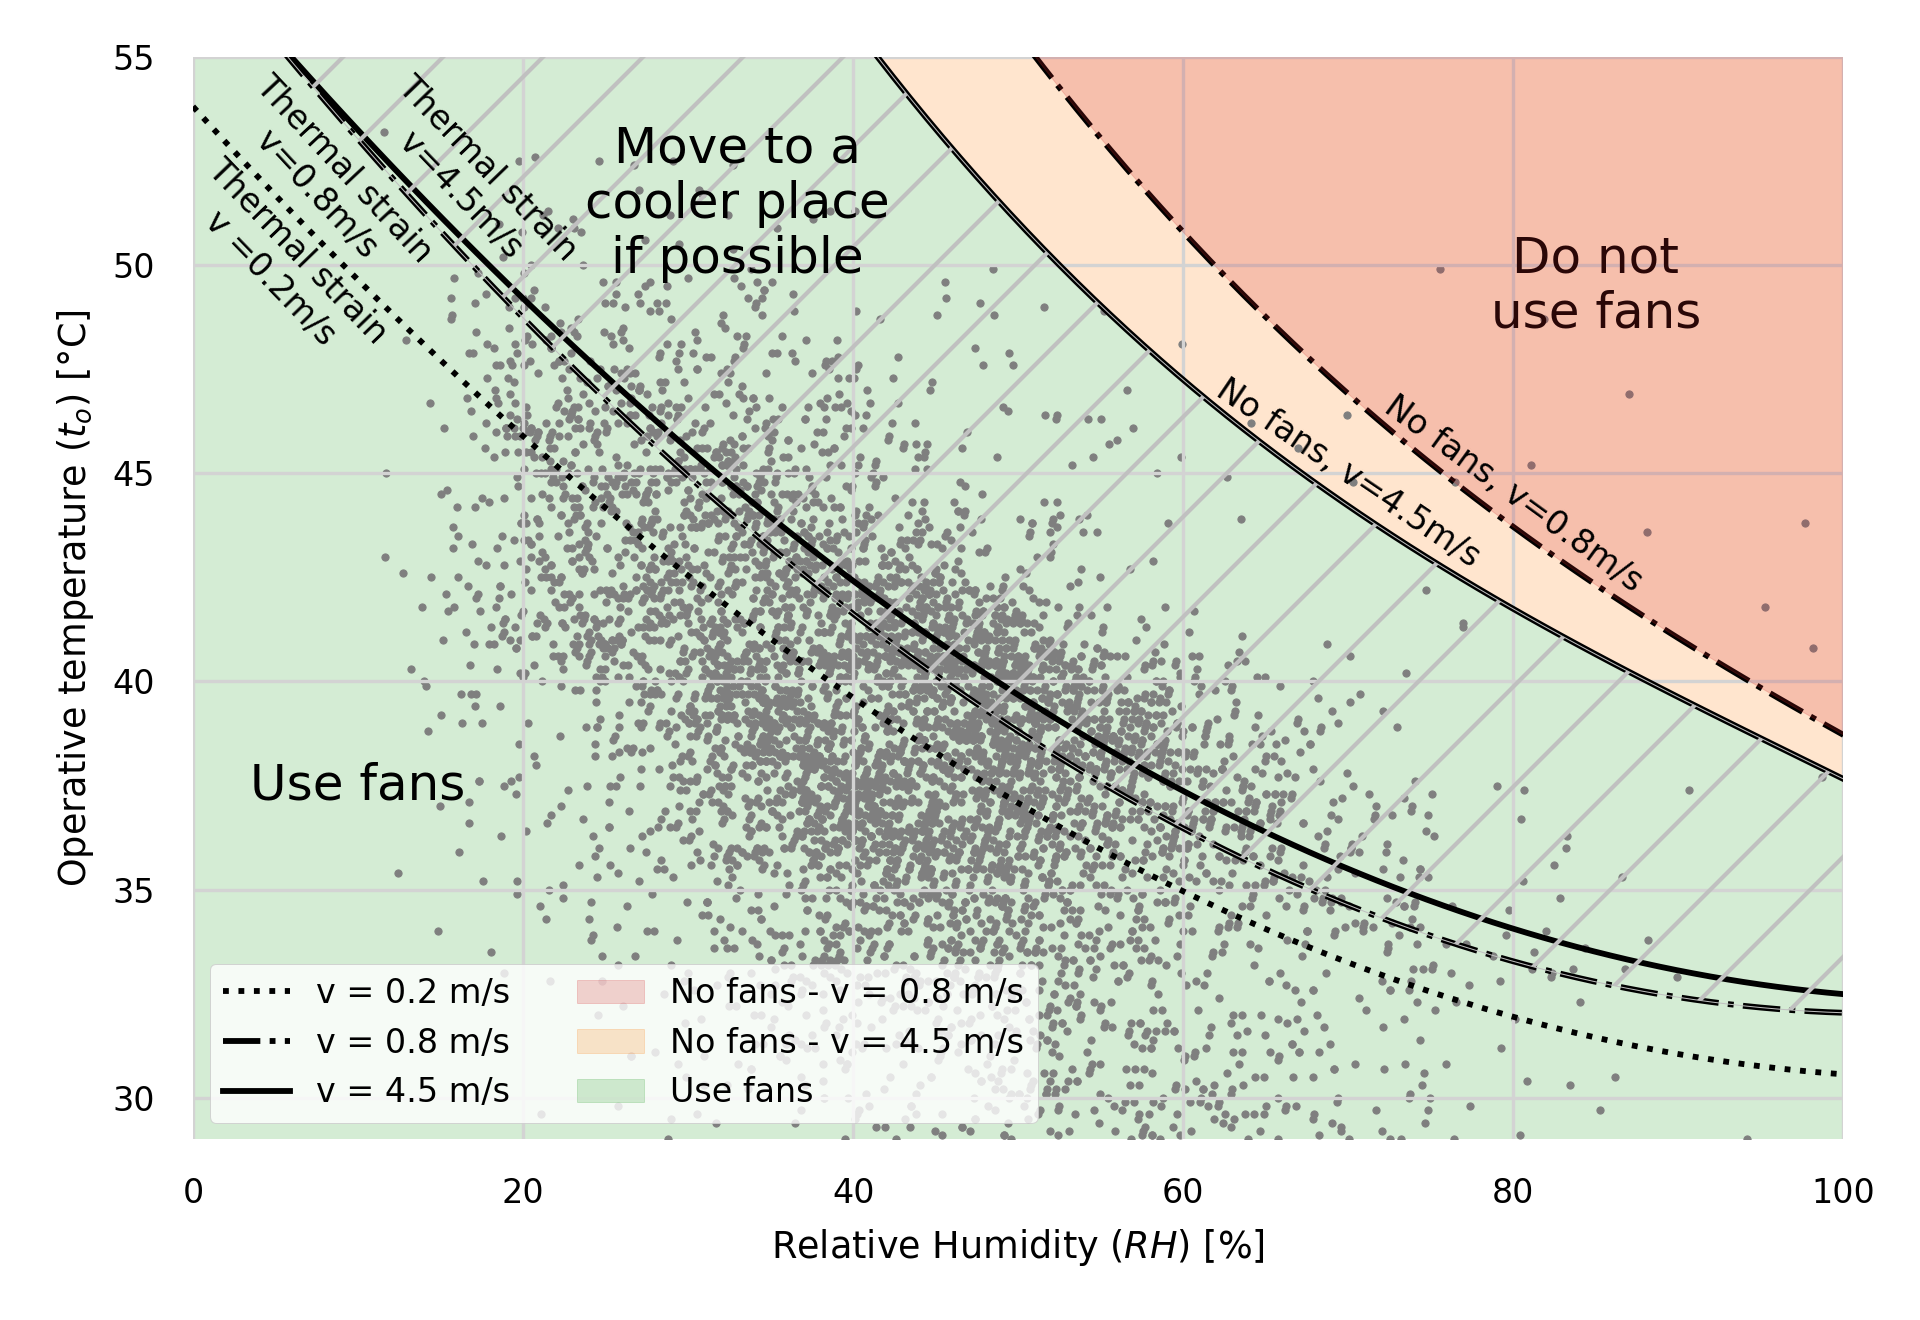
\includegraphics[width=0.75\textwidth]{figures/use_fans}
            \caption{The green area shows the environmental conditions in which the use of fans is beneficial since they provide additional cooling to the human body.
            The dark lines demarcate the regions above which thermal stress is predicted to occur for that specific \ac{v}.
            In the hatched area, while the use of fans it is still beneficial, people are most likely to suffer from heat strain.
            The red area demarcates the region in which electric fans should not be used.
            The dots show the maximum extreme climate conditions recorded over the last 20 years in more than 5000 locations worldwide.
            The red line depicts the current upper temperature limit above which many standards discourage people from using electric fans.}
            \label{fig:energy_storage_delta}
        \end{figure}
    \end{frame}

    \begin{frame}{Results}
        \begin{figure}[thb!]
            \centering
            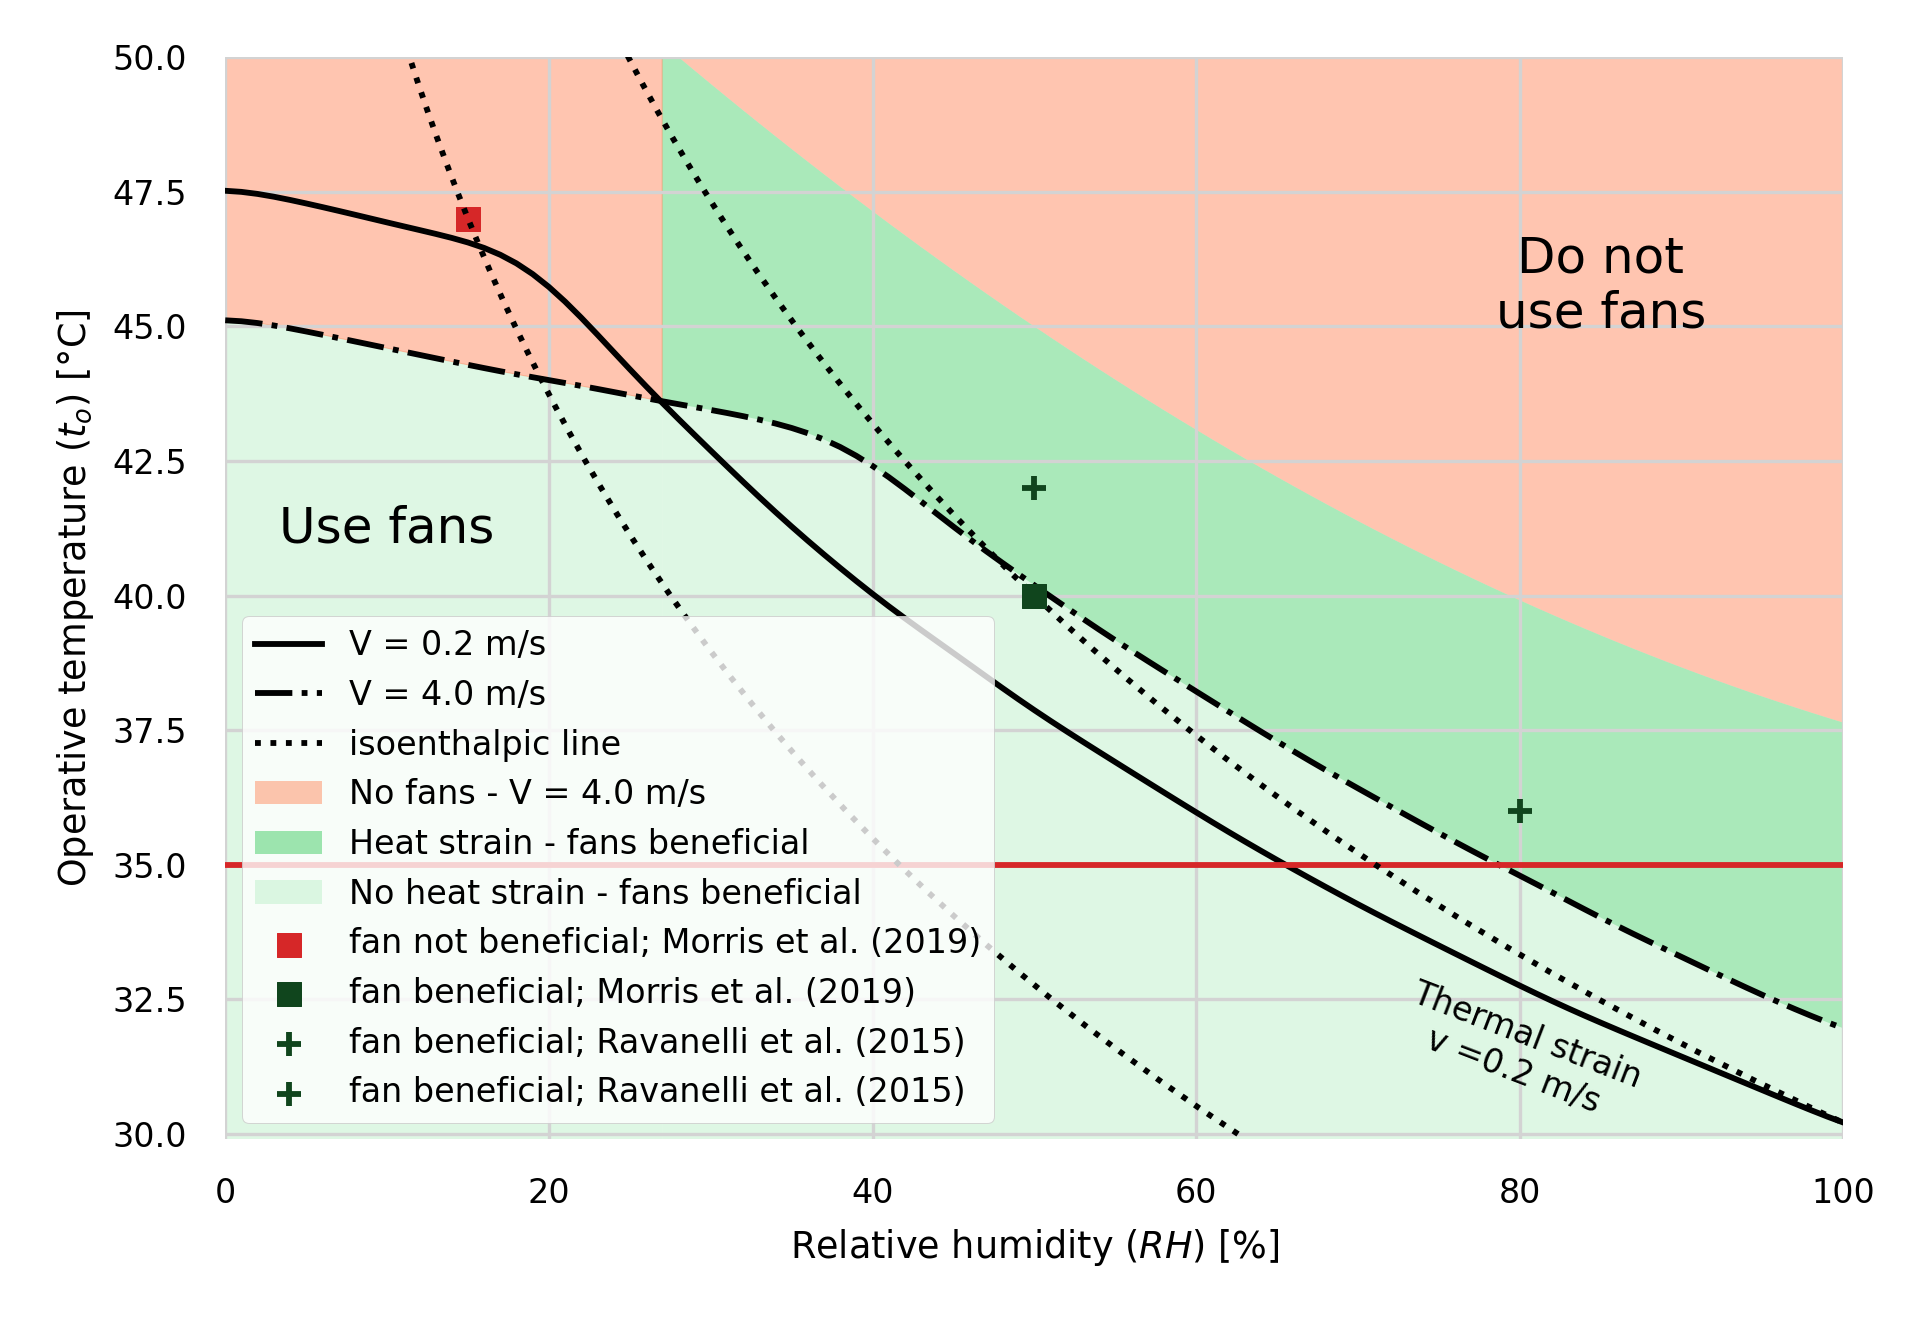
\includegraphics[width=0.75\textwidth]{figures/summary_use_fans_comparison_experimental}
            \caption{Environmental conditions under which the use of electric fans is beneficial, for more information on how to interpret the Figure please refer to the caption of Figure~\ref{fig:energy_storage_delta}
            }
            \label{fig:use_fans_experimental}
        \end{figure}
    \end{frame}

    \begin{frame}{Results}
        \begin{figure}[thb!]
            \centering
            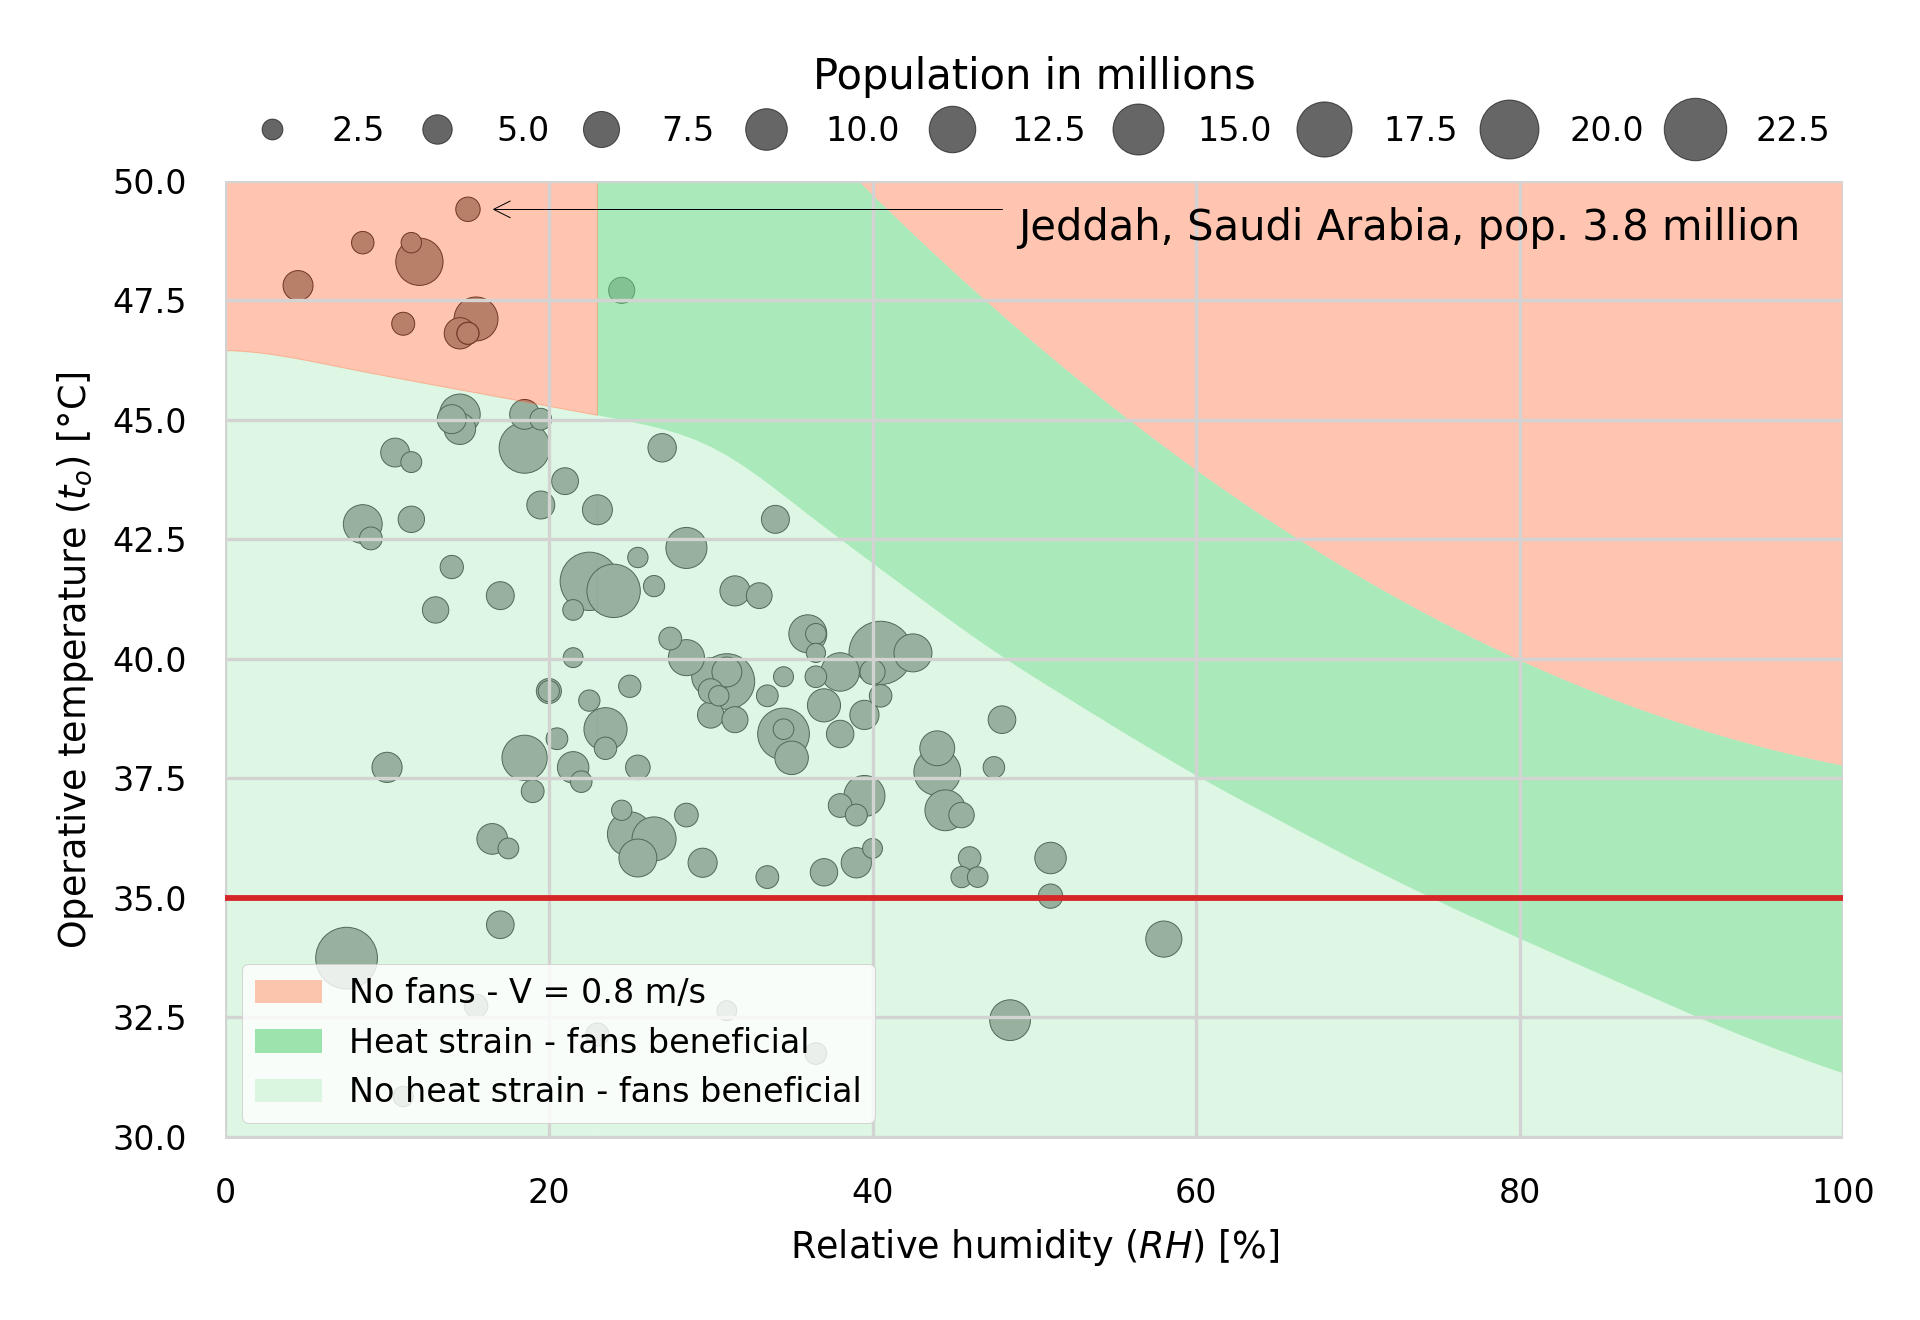
\includegraphics[width=0.75\textwidth]{figures/use_fans_and_population}
            \caption{Environmental conditions under which the use of electric fans is beneficial, for more information on how to interpret the Figure please refer to the caption of Figure~\ref{fig:energy_storage_delta}.
            Each dot shows the maximum extreme climate conditions recorded over the last 20 years in each of the 115 most populous cities worldwide.}
            \label{fig:use_fans_and_population}
        \end{figure}
    \end{frame}uns

    \begin{frame}{Conclusions}
        Electric fans:
        \begin{itemize}
            \item are a cheaper and more energy efficient than air conditioning;
            \item require less energy to operate;
            \item have lower operational and maintenance cost, and do not use refrigerants;
            \item can safely be used when \ac{t-db} exceeds \ac{t-sk}.
        \end{itemize}
    \end{frame}

    \begin{frame}{Conclusions}
        In 2017, 43.6~\% of the world population lived with less than \$5.50 per day, respectively~\cite{PovertyO1:online}.
        They should not be discouraged from using fans when \ac{t-db} exceeds \ac{t-sk}.

        In higher-income countries, low income people, the elderly and people with varying types of physical disabilities are those who are mostly at risk during heatwaves, and may not be able to cool or leave their homes during heatwaves.

        Elevating air speed indoors has the additional benefit of reducing the peak energy demand during.
    \end{frame}

\end{document}